\documentclass[11pt,a4paper]{article}

\usepackage[T1]{fontenc}
\usepackage{lmodern}
\usepackage[a4paper,margin=2.5cm]{geometry}
\usepackage{amsmath,amssymb,amsthm}
\usepackage{booktabs,array}
\usepackage{graphicx}
\usepackage{enumitem}
\usepackage[most]{tcolorbox}
\usepackage[colorlinks=true,linkcolor=blue!50!black,urlcolor=blue!50!black]{hyperref}

% Figures produced by `python -m bs_pricer.demo` (relative to this file).
\graphicspath{{../../results/bs_pricer/}}

\setlength{\parindent}{0pt}
\setlength{\parskip}{0.6em}

% ---------- macros ----------
\newcommand{\E}{\mathbb{E}}
\newcommand{\Q}{\mathbb{Q}}
\newcommand{\npdf}{\varphi}
\newcommand{\dd}{\mathrm{d}}
\newcommand{\fn}[1]{\texttt{\detokenize{#1}}}   % function / file / variable names

\theoremstyle{plain}
\newtheorem*{lemma}{Lemma}
\theoremstyle{remark}
\newtheorem*{remark}{Remark}

% Box used to tie the mathematics back to the source files.
\newtcolorbox{codenote}[1][]{
  breakable, colback=blue!4, colframe=blue!45!black, boxrule=0.5pt,
  arc=2pt, left=6pt, right=6pt, top=4pt, bottom=4pt,
  title={What the code does}, fonttitle=\bfseries\small, #1}

\title{Black--Scholes Pricer\\[0.3em]\large Theory behind each module, and how the code implements it}
\author{\texttt{quant\_models/bs\_pricer}}
\date{\today}

\begin{document}
\maketitle
\tableofcontents

% =====================================================================
\section{Overview and notation}
% =====================================================================

The \fn{bs_pricer} package prices a European option in four independent ways
(closed form, binomial tree, Monte Carlo, and by replicating it with a
delta-hedge), computes its sensitivities, inverts the pricing formula to
recover implied volatility, and finally shows where the model disagrees with
market prices. Each section below states the theory first and then, in a shaded
box, explains what the corresponding code does and why it is written that way.

\subsection*{Notation and conventions}

\begin{center}
\renewcommand{\arraystretch}{1.25}
\begin{tabular}{@{}cll@{}}
\toprule
Symbol & Meaning & Code name \\
\midrule
$S$ & spot price of the underlying & \fn{S} \\
$K$ & strike & \fn{K} \\
$T$ & time to expiry, in years & \fn{T} \\
$r$ & continuously compounded risk-free rate & \fn{r} \\
$q$ & continuous dividend yield (default $0$) & \fn{q} \\
$\sigma$ & volatility of log-returns, per $\sqrt{\text{year}}$ & \fn{sigma} \\
$N(\cdot),\ \npdf(\cdot)$ & standard normal CDF and density & \fn{norm.cdf}, \fn{norm.pdf} \\
$C,\ P$ & European call and put prices & \fn{option_type} \\
\bottomrule
\end{tabular}
\end{center}

The Greeks are returned in \emph{raw} units: vega is per unit (i.e.\ $1.00 = 100$ vol
points) of $\sigma$, theta is per year, and rho is per unit of $r$. To obtain the
familiar quoted units divide by $100$, $365$ and $100$ respectively; the dashboard
does exactly this.

\subsection*{Code map}

\begin{center}
\renewcommand{\arraystretch}{1.25}
\begin{tabular}{@{}p{3.1cm}p{5.3cm}p{5.6cm}@{}}
\toprule
File & Main functions & Theory (section) \\
\midrule
\fn{black_scholes.py} & \fn{vanilla_payoff}, \fn{bs_price}, \fn{bs_delta}, \fn{bs_greeks}, \fn{implied_vol} & Closed form (\ref{sec:closed}), Greeks (\ref{sec:greeks}), implied vol (\ref{sec:iv}) \\
\fn{binomial_tree.py} & \fn{binomial_price} & Binomial tree (\ref{sec:tree}) \\
\fn{monte_carlo.py} & \fn{mc_price} & Monte Carlo (\ref{sec:mc}) \\
\fn{hedging.py} & \fn{delta_hedge_pnl} & Delta hedging (\ref{sec:hedge}) \\
\fn{smile.py} & \fn{smile_from_chain}, \fn{synthetic_smile} & Volatility smile (\ref{sec:smile}) \\
\fn{app.py}, \fn{demo.py} & dashboard and experiments & Section~\ref{sec:glue} \\
\bottomrule
\end{tabular}
\end{center}

% =====================================================================
\section{The model and risk-neutral pricing}
% =====================================================================

\subsection{Geometric Brownian motion}

Black--Scholes assumes the underlying follows
\begin{equation}\label{eq:gbm}
\dd S_t = \mu S_t\,\dd t + \sigma S_t\,\dd W_t ,
\end{equation}
with constant $\mu$ and $\sigma$. By It\^o's lemma,
$\ln S_t$ is Brownian motion with drift $\mu-\tfrac12\sigma^2$, so
\begin{equation}\label{eq:lognormal}
S_T = S_0\exp\!\Big[\big(\mu-\tfrac12\sigma^2\big)T+\sigma\sqrt{T}\,Z\Big],\qquad Z\sim N(0,1).
\end{equation}
The $-\tfrac12\sigma^2$ is the It\^o correction: it is exactly what makes
$\E[S_T]=S_0e^{\mu T}$ rather than something larger. Prices are therefore
\emph{lognormal}, which is why they cannot go negative.

\subsection{Why the real-world drift disappears}

An option can be replicated by trading the underlying and a risk-free bond. Because
the replicating portfolio costs a definite amount, no-arbitrage forces the option to
cost the same. The replication argument eliminates $\mu$ and gives the
Black--Scholes PDE for the option value $V(t,S)$ (with a continuous dividend yield $q$):
\begin{equation}\label{eq:pde}
\frac{\partial V}{\partial t}+\tfrac12\sigma^2S^2\frac{\partial^2 V}{\partial S^2}
+(r-q)S\frac{\partial V}{\partial S}-rV=0,\qquad V(T,S)=\text{payoff}(S).
\end{equation}
Equation~\eqref{eq:pde} is solved equivalently by the \emph{risk-neutral valuation
formula}
\begin{equation}\label{eq:rn}
V_0=e^{-rT}\,\E^{\Q}\big[\text{payoff}(S_T)\big],
\end{equation}
where under $\Q$ the process is~\eqref{eq:gbm} with $\mu$ replaced by $r-q$:
\begin{equation}\label{eq:lognormalQ}
S_T=S_0\exp\!\Big[\big(r-q-\tfrac12\sigma^2\big)T+\sigma\sqrt{T}\,Z\Big].
\end{equation}
This single idea powers three of the four pricing methods in the package: the closed
form evaluates the expectation~\eqref{eq:rn} analytically, Monte Carlo estimates it by
sampling, and the binomial tree evaluates it on a discrete approximation of the
distribution. The fourth (delta hedging) is the replication argument itself.

\subsection{Payoffs}

A European call pays $(S_T-K)^+=\max(S_T-K,0)$ and a put pays $(K-S_T)^+$.

\begin{codenote}
\fn{vanilla_payoff(S, K, option_type)} returns exactly these two payoffs. It uses
\fn{np.maximum}, so \fn{S} can be a single number or an entire array of terminal prices;
this is what lets the tree, the Monte Carlo pricer and the hedging simulator all
share it without loops. Any other option type raises an error.
\end{codenote}

% =====================================================================
\section{The closed-form price}\label{sec:closed}
% =====================================================================

\subsection{Derivation}

Let $F=Se^{(r-q)T}$ be the forward price. From~\eqref{eq:lognormalQ},
$\ln S_T\sim N\big(\ln F-\tfrac12\sigma^2T,\ \sigma^2T\big)$. Define
\begin{equation}\label{eq:d1d2}
d_1=\frac{\ln(S/K)+\big(r-q+\tfrac12\sigma^2\big)T}{\sigma\sqrt T},\qquad
d_2=d_1-\sigma\sqrt T=\frac{\ln(S/K)+\big(r-q-\tfrac12\sigma^2\big)T}{\sigma\sqrt T}.
\end{equation}
For the call, $C=e^{-rT}\big(\E^\Q[S_T\mathbf 1_{\{S_T>K\}}]-K\,\Q(S_T>K)\big)$.

\emph{Second term.} $S_T>K$ is the event $Z>-d_2$, so $\Q(S_T>K)=N(d_2)$.

\emph{First term.} Writing $S_T=F\,e^{\sigma\sqrt T Z-\frac12\sigma^2T}$ and completing the square,
\[
\E^\Q\big[S_T\mathbf 1_{\{S_T>K\}}\big]
= F\int_{-d_2}^{\infty}\npdf\big(z-\sigma\sqrt T\big)\,\dd z
= F\,N\big(d_2+\sigma\sqrt T\big)=F\,N(d_1).
\]
Putting these together,
\begin{equation}\label{eq:bscall}
\boxed{\,C=Se^{-qT}N(d_1)-Ke^{-rT}N(d_2)\,}
\end{equation}
\textbf{Interpretation.} $N(d_2)$ is the risk-neutral probability of finishing in the
money; $Ke^{-rT}N(d_2)$ is the present value of the strike you expect to pay; and
$Se^{-qT}N(d_1)$ is the present value of the share you expect to receive,
\emph{conditional} on exercising (hence $N(d_1)>N(d_2)$: the share is worth more
in the states where you exercise).

\subsection{The put and put--call parity}

Since $(S_T-K)^+-(K-S_T)^+=S_T-K$ for every outcome, taking discounted expectations gives
put--call parity
\begin{equation}\label{eq:parity}
C-P=Se^{-qT}-Ke^{-rT}.
\end{equation}
Combined with $N(x)+N(-x)=1$ this gives
\begin{equation}\label{eq:bsput}
P=Ke^{-rT}N(-d_2)-Se^{-qT}N(-d_1).
\end{equation}

\subsection{Sanity checks}

\begin{itemize}[nosep]
\item As $T\to0$, $C\to(S-K)^+$. As $\sigma\to0$ the call tends to $\max(Se^{-qT}-Ke^{-rT},0)$,
      the discounted intrinsic value. As $\sigma\to\infty$ it tends to $Se^{-qT}$.
      These limits are the no-arbitrage bounds used in Section~\ref{sec:iv}.
\item For the demo contract $S=K=100,\ T=1,\ r=5\%,\ \sigma=20\%$ the formulas give
      $C=10.4506$ and $P=5.5735$; indeed $C-P=4.8771=100-100e^{-0.05}$, as parity requires.
\end{itemize}

\begin{codenote}
\fn{_d1_d2} computes $d_1$ and $d_2$ from~\eqref{eq:d1d2} once, and \fn{bs_price}
reuses them: calls use~\eqref{eq:bscall} and puts use~\eqref{eq:bsput}
(written with $N(-d)$ rather than $1-N(d)$, which is more accurate in the tails).
Everything is written with NumPy operations, so \fn{S} (or any other input) may be an
array and the price is computed for all elements at once. The dividend yield
enters only through the two factors $e^{-qT}$ and the $-q$ in $d_1$. There is no
special handling of $T=0$ or $\sigma=0$: both would divide by zero in $d_1$,
so the function expects $T>0$ and $\sigma>0$.
\end{codenote}

% =====================================================================
\section{The Greeks}\label{sec:greeks}
% =====================================================================

The Greeks are partial derivatives of the price. They quantify the risk of an option
position and, as Section~\ref{sec:hedge} shows, delta and gamma drive hedging.

\subsection{A key identity}

\begin{lemma}
$Se^{-qT}\npdf(d_1)=Ke^{-rT}\npdf(d_2)$.
\end{lemma}
\begin{proof}
$\npdf(d_1)/\npdf(d_2)=\exp\!\big[-\tfrac12(d_1-d_2)(d_1+d_2)\big]$. Now $d_1-d_2=\sigma\sqrt T$ and
$d_1+d_2=2\ln(F/K)/(\sigma\sqrt T)$, so the ratio equals $e^{-\ln(F/K)}=K/F$.
Substituting $F=Se^{(r-q)T}$ gives the claim.
\end{proof}

Whenever $C$ is differentiated, the terms arising from differentiating $N(d_1)$ and
$N(d_2)$ largely cancel because of this lemma. This is why the Greeks are so compact.

\subsection{Derivations for the call}

\textbf{Delta.} $\partial d_1/\partial S=\partial d_2/\partial S=1/(S\sigma\sqrt T)$, so
\[
\frac{\partial C}{\partial S}=e^{-qT}N(d_1)+\underbrace{\big[Se^{-qT}\npdf(d_1)-Ke^{-rT}\npdf(d_2)\big]}_{=0\text{ by the lemma}}\frac{1}{S\sigma\sqrt T}
=e^{-qT}N(d_1).
\]

\textbf{Gamma.} Differentiate once more: $\Gamma=\dfrac{e^{-qT}\npdf(d_1)}{S\sigma\sqrt T}$.

\textbf{Vega.} $\partial d_1/\partial\sigma-\partial d_2/\partial\sigma=\sqrt T$, and the lemma again removes the
$N$-terms, leaving $\mathcal V=Se^{-qT}\npdf(d_1)\sqrt T$.

\textbf{Theta.} Theta is the rate of change with calendar time, $\Theta=-\partial C/\partial T$.
Using the lemma and $\partial(d_1-d_2)/\partial T=\sigma/(2\sqrt T)$,
\[
\Theta_C=-\frac{Se^{-qT}\npdf(d_1)\,\sigma}{2\sqrt T}-rKe^{-rT}N(d_2)+qSe^{-qT}N(d_1).
\]

\textbf{Rho.} Only the discount factor survives: $\rho_C=KTe^{-rT}N(d_2)$.

\subsection{The put, from parity}

Differentiating~\eqref{eq:parity} shows that the put and call share gamma and vega, and
\begin{align*}
\Delta_P&=\Delta_C-e^{-qT}=e^{-qT}\big(N(d_1)-1\big), \\
\Theta_P&=-\frac{Se^{-qT}\npdf(d_1)\sigma}{2\sqrt T}+rKe^{-rT}N(-d_2)-qSe^{-qT}N(-d_1), \\
\rho_P&=-KTe^{-rT}N(-d_2).
\end{align*}

\subsection{Interpretation and a consistency check}

\begin{center}
\renewcommand{\arraystretch}{1.3}
\begin{tabular}{@{}lll@{}}
\toprule
Greek & Meaning & Sign / shape \\
\midrule
Delta $\Delta$ & price change per unit move in $S$; hedge ratio & call $\in(0,e^{-qT})$, put $\in(-e^{-qT},0)$ \\
Gamma $\Gamma$ & change of delta per unit move in $S$ & positive, peaks near the strike \\
Vega $\mathcal V$ & price change per unit move in $\sigma$ & positive, same for call and put \\
Theta $\Theta$ & price change as time passes & usually negative (time decay) \\
Rho $\rho$ & price change per unit move in $r$ & call positive, put negative \\
\bottomrule
\end{tabular}
\end{center}

The Greeks are not independent. Substituting them into~\eqref{eq:pde} gives
\begin{equation}\label{eq:thetagamma}
\Theta+\tfrac12\sigma^2S^2\Gamma+(r-q)S\Delta=rV .
\end{equation}
For a delta-hedged position ($\Delta$ neutralised), this says time decay is paid for by
gamma: $\Theta\approx-\tfrac12\sigma^2S^2\Gamma$ (plus a small $rV$ financing term). This
``theta--gamma trade-off'' is the heart of the hedging experiment.
For the demo call ($S=K=100$, $T=1$, $r=5\%$, $\sigma=20\%$):
$\Delta=0.6368$, $\Gamma=0.01876$, $\mathcal V=37.52$ (i.e.\ $0.375$ per vol point),
$\Theta=-6.414$ per year ($-0.0176$ per day), $\rho=53.23$ ($0.532$ per 1\% rate move), and
equation~\eqref{eq:thetagamma} holds to within rounding:
$-6.4140+3.7524+3.1842-0.5225\approx0$.

\begin{codenote}
\fn{bs_delta} is a separate function because hedging calls it thousands of times and
needs nothing else. \fn{bs_greeks} computes $d_1,d_2$, the density
$\npdf(d_1)$ and the two discount factors $e^{-qT},e^{-rT}$ once, then forms
gamma and vega (identical for calls and puts) directly. The variable \fn{decay}
is the common first term of theta, $-Se^{-qT}\npdf(d_1)\sigma/(2\sqrt T)$; the call
and put branches then add their own $r$- and $q$-dependent terms exactly as in the
formulas above, and compute rho. The result is returned as a dictionary of
arrays with keys \fn{delta, gamma, vega, theta, rho}. Because everything is vectorised,
the dashboard can evaluate a whole range of spot prices in one call to draw the
Greek-versus-spot curves.
\end{codenote}

% =====================================================================
\section{Implied volatility}\label{sec:iv}
% =====================================================================

\subsection{Definition and existence}

Of the model inputs, $\sigma$ is the only one that cannot be observed. Given an
observed market price $P^\ast$, the \emph{implied volatility} is the $\sigma$ solving
\begin{equation}\label{eq:iv}
\mathrm{BS}(S,K,T,r,q,\sigma)=P^\ast .
\end{equation}
Since vega is strictly positive for $T>0$, the map $\sigma\mapsto\mathrm{BS}$ is
strictly increasing, so there is at most one solution. Its range, as $\sigma$ runs over
$(0,\infty)$, is the open interval between the no-arbitrage bounds:
\[
\begin{aligned}
\text{call: }&\ \max\!\big(Se^{-qT}-Ke^{-rT},0\big)<C<Se^{-qT},\\
\text{put: }&\ \max\!\big(Ke^{-rT}-Se^{-qT},0\big)<P<Ke^{-rT}.
\end{aligned}
\]
A solution exists if and only if the quote lies strictly inside these bounds; otherwise no
Black--Scholes volatility can reproduce it.

\subsection{Newton--Raphson}

Newton's method applied to $f(\sigma)=\mathrm{BS}(\sigma)-P^\ast$, whose derivative is vega, iterates
\begin{equation}\label{eq:newton}
\sigma_{k+1}=\sigma_k-\frac{\mathrm{BS}(\sigma_k)-P^\ast}{\mathcal V(\sigma_k)} .
\end{equation}
Near the root convergence is quadratic (the number of correct digits roughly doubles per step),
so typically fewer than ten iterations are needed. But Newton can fail, and the reason
is the shape of the price in $\sigma$. Differentiating vega gives $\partial\mathcal V/\partial\sigma=\mathcal V\,d_1d_2/\sigma$, so the
price is \emph{convex} in $\sigma$ while $\sigma<\sigma^\ast=\sqrt{2|\ln(F/K)|/T}$ and \emph{concave} beyond it. For
deep in- or out-of-the-money options the price curve is nearly flat at small $\sigma$ (vega $\approx0$), so a Newton
step divides by a tiny number and can jump to a negative or absurdly large volatility.

\subsection{Bisection}

Bisection only needs the root to be bracketed. Starting from $[\sigma_{\text{lo}},\sigma_{\text{hi}}]$ with
$\mathrm{BS}(\sigma_{\text{lo}})<P^\ast<\mathrm{BS}(\sigma_{\text{hi}})$, repeatedly evaluate the midpoint and keep the half that still
brackets the root. The interval halves each time, so reaching width $\varepsilon$ from width $w$ takes $\log_2(w/\varepsilon)$ steps
(about $29$ for $w=5$, $\varepsilon=10^{-8}$). It converges linearly but \emph{cannot} fail, because monotonicity guarantees
that the bracket is valid.

\begin{codenote}
\fn{implied_vol} follows a ``fast, then safe'' strategy:
\begin{enumerate}[nosep,leftmargin=*]
\item \textbf{Lower-bound check.} It computes the discounted intrinsic value
  $\max(\pm(Se^{-qT}-Ke^{-rT}),0)$ and returns \fn{NaN} if the price is below it.
\item \textbf{Newton phase.} It starts at $\sigma=0.2$ and applies~\eqref{eq:newton}, using
  \fn{bs_greeks} for vega, for at most 50 iterations. It stops successfully when the
  \emph{price} error is below the tolerance (default $10^{-8}$). It abandons Newton if vega falls
  below $10^{-10}$ or if a step would leave $(0,5]$.
\item \textbf{Bisection phase.} On the bracket $[10^{-6},5]$ (i.e.\ up to 500\% volatility). If the target price is
  outside the prices at the two ends of the bracket, the quote is rejected with \fn{NaN}; this is also how
  prices above the upper no-arbitrage bound are caught. Otherwise it bisects for at most 200 steps, stopping when the
  \emph{volatility} interval is narrower than the tolerance, and returns the midpoint.
\end{enumerate}
Note that the two phases measure convergence differently (price error versus volatility error); at
$10^{-8}$ either is far below any market-data noise. The function handles one price at a time (scalars) because it
branches with ordinary \fn{if} statements.
\end{codenote}

% =====================================================================
\section{The binomial tree}\label{sec:tree}
% =====================================================================

\subsection{Construction (Cox--Ross--Rubinstein)}

Divide $[0,T]$ into $n$ steps of length $\Delta t=T/n$. In each step the price multiplies by $u$ (up) or $d$ (down). CRR choose
\begin{equation}\label{eq:crr}
u=e^{\sigma\sqrt{\Delta t}},\qquad d=\frac1u,
\end{equation}
so the tree \emph{recombines} (an up followed by a down returns to the start), giving only $n+1$ distinct terminal nodes
instead of $2^n$. After $i$ steps with $j$ down-moves, $S_{i,j}=Su^{\,i-j}d^{\,j}=Se^{\sigma\sqrt{\Delta t}\,(i-2j)}$.

\textbf{Risk-neutral probability.} The up-probability $p$ is fixed by requiring that the discounted
stock is a martingale, i.e.\ that the one-step expected growth equals $e^{(r-q)\Delta t}$:
\begin{equation}\label{eq:p}
pu+(1-p)d=e^{(r-q)\Delta t}\quad\Longrightarrow\quad p=\frac{e^{(r-q)\Delta t}-d}{u-d}.
\end{equation}
This is the same no-arbitrage argument as in Section~\ref{sec:closed}, in a one-period model: the option can be replicated
by shares and bonds, and the replication cost equals the $p$-weighted discounted payoff. For $p$ to be a probability,
$d<e^{(r-q)\Delta t}<u$, which holds once $n$ is large enough.

\textbf{Why this matches Black--Scholes.} Writing $m=e^{(r-q)\Delta t}$ and $a=\sigma\sqrt{\Delta t}$, one finds
$\E^\Q[(S'/S)^2]=2m\cosh a-1$, hence the one-step variance of the return is
$2m\cosh a-1-m^2=\sigma^2\Delta t+O(\Delta t^2)$.
The tree therefore matches the mean and (to leading order) the variance of the lognormal
dynamics in every step, and by the central limit theorem the terminal distribution converges to the lognormal law~\eqref{eq:lognormalQ}.

\subsection{Backward induction}

At expiry the node values are the payoffs. Stepping backward, each node is the discounted risk-neutral expectation of its two children:
\begin{equation}\label{eq:backward}
V_{i,j}=e^{-r\Delta t}\big[\,p\,V_{i+1,j}+(1-p)\,V_{i+1,j+1}\big],
\end{equation}
where $V_{i+1,j}$ is the up-child and $V_{i+1,j+1}$ the down-child. The price is $V_{0,0}$.

\textbf{American options.} An American holder may exercise at any time, so at each node the value is the larger of continuing and exercising:
\begin{equation}\label{eq:american}
V_{i,j}=\max\!\Big(e^{-r\Delta t}\big[pV_{i+1,j}+(1-p)V_{i+1,j+1}\big],\ \text{payoff}(S_{i,j})\Big).
\end{equation}
There is no closed form for the American put, which is the main reason to use a tree. With no dividends an American call is never
exercised early (its value always exceeds $S-K$), so it equals the European call; an American put can be worth strictly more.
For the demo parameters a 500-step tree gives a European put of $5.5695$ (closed form $5.5735$) and an American put of $6.0888$: the
difference of about $0.52$ is the \emph{early-exercise premium}.

\subsection{Convergence}

The price error shrinks like $1/n$. For the at-the-money demo contract this appears as a clean straight line of slope $-1$ on a log--log
plot (Figure~\ref{fig:conv}); for other strikes the error is known to oscillate in a saw-tooth pattern, depending on where the strike falls
relative to the terminal lattice, while keeping the same overall rate. The cost grows like $n^2$ (about $n^2/2$ node updates). With 500 steps the tree price of the
demo call is $10.4466$, against $10.4506$ in closed form.

\begin{codenote}
\fn{binomial_price} first computes $\Delta t$, $u$, $d$, $p$ and the one-step discount factor.
It builds the vector of terminal stock prices $Su^{\,n-j}d^{\,j}$ for $j=0,\dots,n$ ($j$ counts down-moves) and applies
\fn{vanilla_payoff} to get the terminal option values in one shot. A loop then walks back from step $n-1$ to $0$. In each pass,
the new value vector is the discounted combination of ``this node's up-child'' (\fn{values[:-1]}) and ``its down-child'' (\fn{values[1:]}),
which implements~\eqref{eq:backward} for all nodes of that level at once; the vector shrinks by one element per pass until
only the root remains. If \fn{american=True}, the loop also rebuilds that level's stock prices and takes the elementwise
maximum with the immediate-exercise payoff, i.e.~\eqref{eq:american}. No full tree is stored, only the current level.
\end{codenote}

% =====================================================================
\section{Monte Carlo}\label{sec:mc}
% =====================================================================

\subsection{Estimator}

Because~\eqref{eq:rn} is an expectation, it can be estimated by an average. For a European option only the terminal
price matters, and $S_T$ is known exactly in distribution from~\eqref{eq:lognormalQ}, so no time-stepping error is introduced.
Draw $Z_1,\dots,Z_N$ i.i.d.\ $N(0,1)$, form $S_T^{(i)}$, and set
\begin{equation}\label{eq:mc}
\hat V=\frac1N\sum_{i=1}^N Y_i,\qquad Y_i=e^{-rT}\,\text{payoff}\big(S_T^{(i)}\big).
\end{equation}
$\hat V$ is unbiased, and by the law of large numbers it converges to the true price.

\subsection{Error}

By the central limit theorem $\hat V$ is approximately normal around the truth with standard deviation $s/\sqrt N$, where
$s$ is the standard deviation of the $Y_i$. It is estimated by the sample standard deviation $\hat s$ (with the $N-1$ correction), giving the \emph{standard error}
\begin{equation}\label{eq:se}
\mathrm{SE}=\frac{\hat s}{\sqrt N}.
\end{equation}
A 95\% confidence interval is $\hat V\pm1.96\,\mathrm{SE}$ (the code and demo use the rounder $2\,\mathrm{SE}$). The
important consequence is the \emph{slow} rate $N^{-1/2}$: ten times more accuracy needs a hundred times more paths. In exchange, the
error does not depend on the dimension of the problem, which is why Monte Carlo is the method of choice for path-dependent and
multi-asset options (see the \fn{mc_exotics} package).

\begin{remark}
In the demo (500\,000 paths, seed 1) the estimate is $10.4003$ with $\mathrm{SE}=0.0208$, which is about $2.4$ standard errors
below the exact $10.4506$. A correct unbiased estimator lands that far out for fewer than 2\% of seeds, so one run is a draw from the error
distribution and neither confirms nor refutes the method; the convergence plot, which averages the behaviour over several $N$,
is the better evidence.
\end{remark}

\begin{codenote}
\fn{mc_price} creates a seeded random generator (so results are reproducible), draws \fn{n_paths} standard normals and maps
them to terminal prices through~\eqref{eq:lognormalQ}, i.e.\ with drift $r-q-\tfrac12\sigma^2$ (note: the risk-free rate, not a real-world drift).
It applies the payoff, discounts by $e^{-rT}$, and returns the pair (sample mean, sample standard deviation divided by
$\sqrt N$), matching~\eqref{eq:mc} and~\eqref{eq:se}. The whole computation is vectorised and uses a single sampled step per path.
No variance-reduction technique is applied here; the plain estimator is the point of this module.
\end{codenote}

\begin{figure}[ht]
\centering
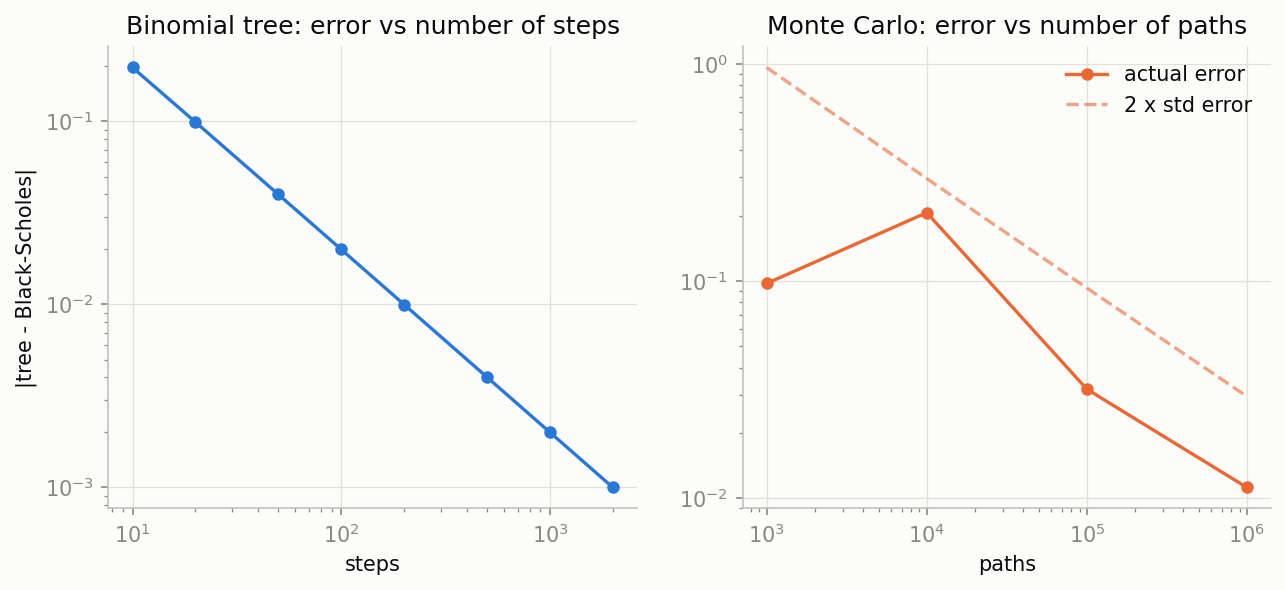
\includegraphics[width=0.95\textwidth]{convergence.png}\label{fig:conv}
\caption{Convergence of the tree (left: a straight line of slope $-1$ on log--log axes, i.e.\ error $\propto1/n$) and
Monte Carlo (right: the error is erratic at small $N$ but trends down like $N^{-1/2}$ and stays below the dashed $2\times$ standard-error band).}
\end{figure}

% =====================================================================
\section{Delta hedging}\label{sec:hedge}
% =====================================================================

\subsection{Replication in continuous time}

The derivation of~\eqref{eq:pde} rests on this fact: if you sell an option for $V$ and continuously hold $\Delta=\partial V/\partial S$ shares,
financing the rest at rate $r$, the random terms cancel and the portfolio ends up worth exactly the payoff you owe. The seller
earns zero profit in every scenario. In practice one can only rebalance at discrete dates, so a hedging error remains.

\subsection{The error of one discrete step}

Take $q=0$ (the simulator has no dividend input). Over one step of length $\Delta t$, a seller who is short the option and long $\Delta=V_S$
shares, with the remainder $B=V-\Delta S$ in cash earning $r$, gains approximately
\[
-\delta V+\Delta\,\delta S+rB\,\Delta t,\qquad \delta V\approx V_t\Delta t+V_S\,\delta S+\tfrac12V_{SS}(\delta S)^2 ,
\]
where $\delta S$ and $\delta V$ denote the changes in $S$ and $V$ over the step.
Using the PDE~\eqref{eq:pde} to eliminate $V_t$, everything cancels except the second-order terms:
\begin{equation}\label{eq:hedgeerr}
\text{P\&L}_{\text{step}}\;\approx\;\tfrac12\,\Gamma\,S^2\Big(\sigma^2\Delta t-\Big(\frac{\delta S}{S}\Big)^2\Big).
\end{equation}
This is the theta--gamma trade-off of~\eqref{eq:thetagamma} made concrete. The seller is \emph{paid} gamma decay $\tfrac12\sigma^2S^2\Gamma\Delta t$
per step by holding the option short, and \emph{loses} $\tfrac12\Gamma S^2(\delta S/S)^2$ to realised movement. The two cancel
on average when realised volatility equals the $\sigma$ used to price and hedge, and the seller loses if the market realises more volatility than $\sigma$.

\subsection{Why the error shrinks like $1/\sqrt n$}

If the realised volatility is $\sigma$, then $(\delta S/S)^2=\sigma^2\Delta t\,Z^2+O(\Delta t^{3/2})$ with $Z\sim N(0,1)$, whatever the drift. Hence
\[
\text{P\&L}_{\text{step}}\approx\tfrac12\Gamma S^2\sigma^2\Delta t\,(1-Z^2),
\]
a zero-mean term of size $O(\Delta t)$ with variance $\tfrac12(\Gamma S^2\sigma^2\Delta t)^2$. Summing $n=T/\Delta t$ roughly independent
steps gives a total variance of order $n\,\Delta t^2=T\Delta t=T^2/n$, so the standard deviation scales as $1/\sqrt n$.
Two further consequences: the error is concentrated where $\Gamma S^2$ is large (near the strike, close to expiry), and the real-world drift $\mu$ does \emph{not}
affect the leading-order result, because the hedge removes the exposure to the direction of the stock.

\subsection{The simulation}

With $n$ hedge dates $t_i=i\Delta t$, $i=0,\dots,n-1$, and $B_i$ the cash account just after the trade at $t_i$:
\begin{align*}
B_0&=V_0-\Delta_0S_0,\\
B_i&=B_{i-1}e^{r\Delta t}-(\Delta_i-\Delta_{i-1})S_i,\qquad \Delta_i=\Delta\big(S_i,\,T-t_i\big),\\
\text{P\&L}&=B_{n-1}e^{r\Delta t}+\Delta_{n-1}S_T-\text{payoff}(S_T).
\end{align*}
The result is the seller's profit measured in money at expiry, starting from zero net investment.

\begin{codenote}
\fn{delta_hedge_pnl} proceeds in four steps.
\begin{enumerate}[nosep,leftmargin=*]
\item \textbf{Simulate paths.} All \fn{n_paths} stock paths are generated at once on the grid of \fn{n_steps} dates using the exact lognormal
  increment $(\mu-\tfrac12\sigma^2)\Delta t+\sigma\sqrt{\Delta t}\,Z$ with cumulative sums, producing an array of shape (paths, steps $+1$).
  The drift \fn{mu} is the \emph{real-world} drift (default $r$); the demo uses $10\%$ against $r=5\%$ to show the hedge does not depend on it.
\item \textbf{Day 0.} The option is sold at its Black--Scholes price, the initial delta is bought, and the cash balance is the
  premium minus the cost of the shares (negative, i.e.\ borrowed).
\item \textbf{Rebalance.} At each date $1,\dots,n-1$ the cash account first accrues interest for one step, then delta is recomputed from the new
  spot and the \emph{remaining} time $T-i\Delta t$, and the difference in shares is bought or sold, with the cash balance adjusted.
  The final date only settles.
\item \textbf{Settle.} After the last interest accrual, the value is cash plus the shares held, minus the option payoff owed. One P\&L number is
  returned per path.
\end{enumerate}
The same $\sigma$ drives the simulation and the hedge, so the experiment isolates \emph{discretisation} error. Running it with a different hedging
volatility would add the systematic term in~\eqref{eq:hedgeerr}.
\end{codenote}

\subsection{Results}

For the demo call (5\,000 paths, $\mu=10\%$) the mean P\&L is close to zero in every case and the spread falls as predicted:

\begin{center}
\renewcommand{\arraystretch}{1.2}
\begin{tabular}{@{}lccc@{}}
\toprule
Rebalancing & Hedges $n$ & Std.\ of P\&L & Std.\ $\times\sqrt n$ \\
\midrule
Quarterly & 4 & 3.13 & 6.25 \\
Monthly & 12 & 1.89 & 6.55 \\
Weekly & 52 & 0.92 & 6.61 \\
Daily & 252 & 0.43 & 6.75 \\
\bottomrule
\end{tabular}
\end{center}
The last column is nearly constant, confirming the $1/\sqrt n$ law. Even daily hedging does not remove the risk entirely.

\begin{figure}[ht]
\centering
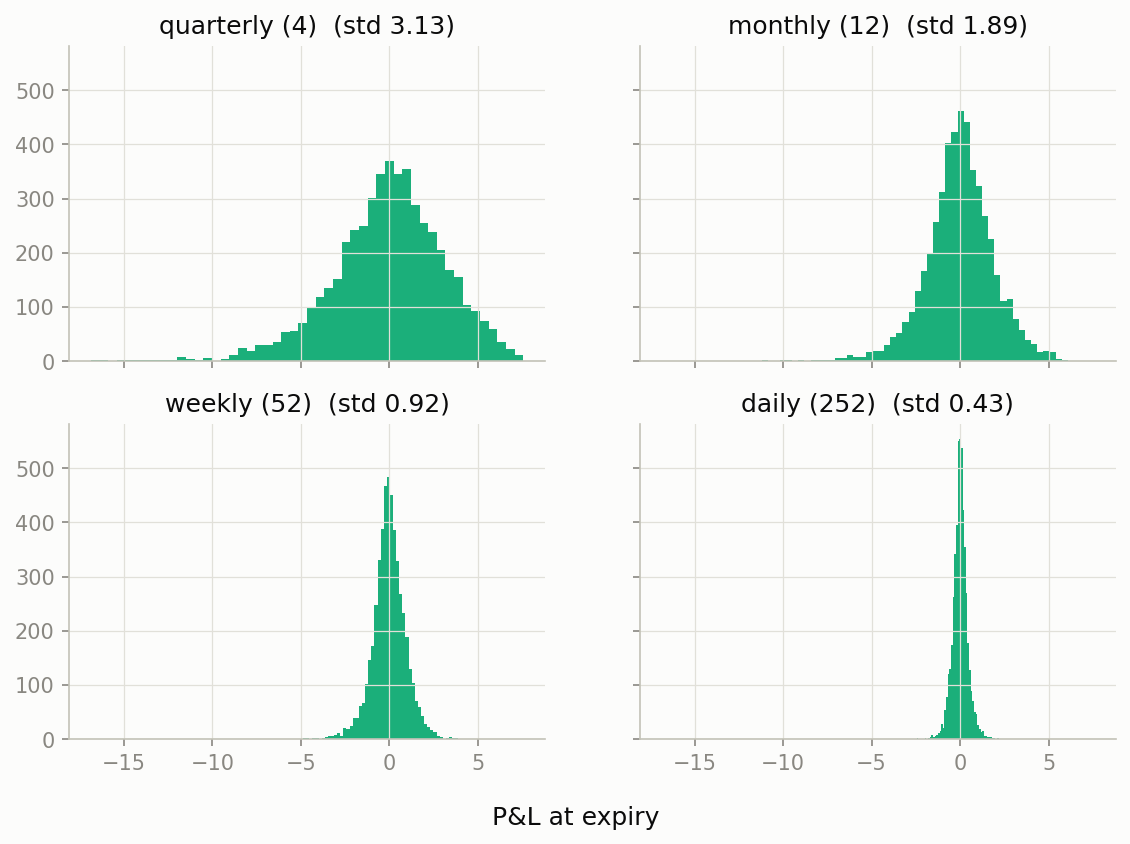
\includegraphics[width=0.8\textwidth]{delta_hedging.png}
\caption{Distribution of the terminal P\&L of a delta-hedged short call at four rebalancing frequencies.}
\end{figure}

% =====================================================================
\section{The volatility smile}\label{sec:smile}
% =====================================================================

\subsection{The phenomenon}

If Black--Scholes were true, one volatility would reproduce every option on the same underlying and expiry. Instead, inverting market prices
via~\eqref{eq:iv} gives a different implied volatility for each strike. Equity-index options typically show a \emph{skew}: low strikes
(downside protection) have higher implied volatility than high strikes; individual equities and currencies show more symmetric \emph{smiles}.

Implied volatility is best understood as a \emph{quoting convention}, a way of expressing a price in units that are easier to compare across strikes
and maturities, rather than a literal forecast of volatility. Its dependence on strike is evidence against the model's assumptions:
\begin{itemize}[nosep]
\item returns have fatter tails than a normal distribution, which raises the price of far out-of-the-money options relative to the model;
\item volatility is not constant: it is stochastic and tends to rise when prices fall (the leverage effect), which produces the downside skew;
\item prices can jump, and there is persistent demand for crash protection.
\end{itemize}
Stochastic-volatility (e.g.\ Heston) and jump models were developed to reproduce this surface.

\subsection{Which options to use}

Smile construction uses only out-of-the-money options: puts below the spot and calls above it. They are the most actively traded, so their
quotes are the most reliable. For listed American-style options (such as SPY) in-the-money prices also contain an early-exercise premium which
Black--Scholes does not model, and for European options parity~\eqref{eq:parity} means they carry no information beyond the out-of-the-money
option at the same strike. The sensitivity of an inferred volatility to a price error is approximately $\delta\sigma\approx\delta P/\mathcal V$, so quotes on
low-vega options give noisy implied volatilities, which motivates filtering.

\begin{codenote}
\fn{smile_from_chain} downloads an option chain through \fn{yfinance} for the first expiry at least \fn{min_days} (default 20)
away, taking the spot from the latest close. For each quote it keeps calls with strike at or above spot and puts with strike below spot, skips quotes with a zero
bid or ask, uses the \emph{mid-price} $\tfrac12(\text{bid}+\text{ask})$ as the market price, converts days to years by dividing by 365,
and calls \fn{implied_vol}. Results outside $1\%<\sigma<300\%$ or non-finite are discarded as bad data. If anything fails (no network,
no options listed) it prints the error and returns \fn{None}, and the demo falls back to the synthetic smile.

The rate is a flat 4\% and the dividend yield is left at zero, so the numbers are approximate: SPY pays a dividend and its options are American-style.

\fn{synthetic_smile} runs the process in reverse as a self-test. It defines a known volatility curve in log-moneyness $x=\ln(K/S)$,
$\sigma(x)=0.20-0.25\,x+0.6\,x^2$ (a downward skew with some curvature), prices options from it using \fn{bs_price}, and then recovers the volatilities
with \fn{implied_vol}. If the recovered points lie on the known curve, the implied-volatility solver round-trips correctly.
\end{codenote}

\begin{figure}[ht]
\centering
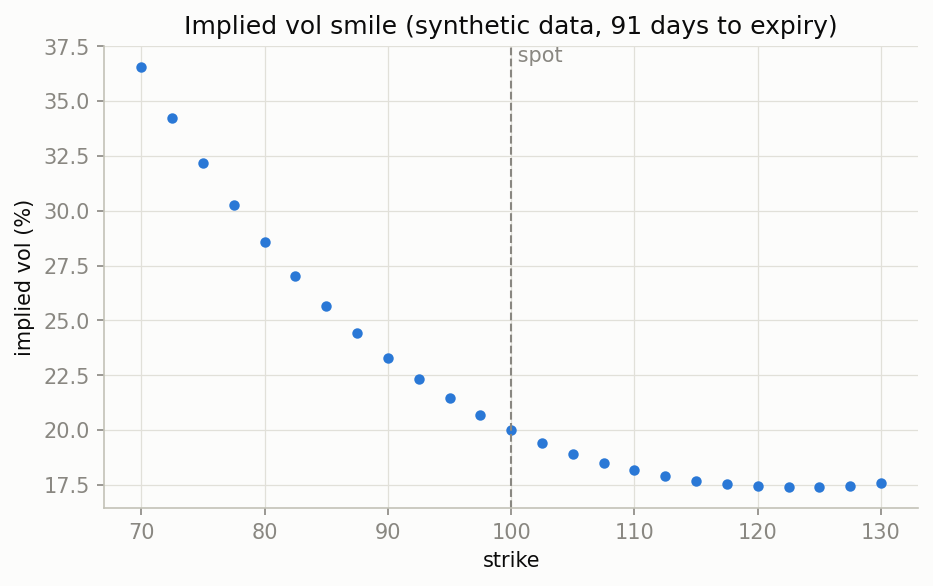
\includegraphics[width=0.7\textwidth]{vol_smile.png}
\caption{Implied volatility versus strike for the synthetic smile (91 days to expiry). The curve falls steeply for low strikes and flattens above spot.}
\end{figure}

% =====================================================================
\section{How the pieces connect: dashboard and demo}\label{sec:glue}
% =====================================================================

\textbf{Dashboard (\fn{app.py}).} A Streamlit page whose sliders feed $(S,K,T,r,\sigma)$ to \fn{bs_price}, \fn{binomial_price} (300 steps)
and \fn{mc_price} ($10^5$ paths), showing the three prices side by side (the Monte Carlo price is shown with a $\pm2\,\mathrm{SE}$ band). It displays the Greeks converted to the market
units above, and plots the price or any Greek against spot over $[0.5K,1.5K]$ by passing an array of spots to the vectorised functions.

\textbf{Demo (\fn{demo.py}).} Runs four experiments and saves the figures: the three prices and Greeks of the reference call; convergence of tree error versus steps and
Monte Carlo error versus paths; the hedging histograms; and the smile.

For the reference call the methods agree as follows:
\begin{center}
\renewcommand{\arraystretch}{1.2}
\begin{tabular}{@{}lcc@{}}
\toprule
Method & Price & Note \\
\midrule
Closed form & 10.4506 & exact within the model \\
Binomial tree, 500 steps & 10.4466 & error $\approx 4\times10^{-3}$ \\
Monte Carlo, $5\times10^5$ paths, seed 1 & 10.4003 & $\mathrm{SE}=0.0208$ \\
\bottomrule
\end{tabular}
\end{center}

% =====================================================================
\section{Assumptions and limitations}
% =====================================================================

Each Black--Scholes assumption has a visible consequence in this package:

\begin{center}
\renewcommand{\arraystretch}{1.25}
\begin{tabular}{@{}p{4.2cm}p{6cm}p{4cm}@{}}
\toprule
Assumption & What goes wrong in practice & Where it shows \\
\midrule
Constant $\sigma$ & implied volatility varies with strike and expiry & smile (Sec.~\ref{sec:smile}) \\
Continuous, costless trading & discrete hedging leaves residual risk; costs make it worse & hedging (Sec.~\ref{sec:hedge}) \\
Lognormal prices, no jumps & fat tails and gaps & smile, hedging error \\
Constant $r$ and $q$ & rates and dividends vary; discrete dividends & flat 4\% rate in the smile code \\
European exercise & listed equity options are usually American & tree comparison; SPY smile \\
\bottomrule
\end{tabular}
\end{center}

\textbf{Edge cases worth knowing about in the code.}
\begin{itemize}[nosep]
\item \fn{bs_price}, \fn{bs_greeks} and \fn{bs_delta} require $T>0$ and $\sigma>0$ (they divide by $\sigma\sqrt T$).
\item \fn{delta_hedge_pnl} has no dividend-yield argument, so it hedges a non-dividend-paying asset.
\item \fn{implied_vol} accepts scalars only, searches $\sigma\in[10^{-6},5]$, and returns \fn{NaN} for prices outside the no-arbitrage range, or at its very edge.
\item Monte Carlo and the hedging simulator are reproducible only because they take a seed.
\end{itemize}

\textbf{Natural extensions} follow from the above: stochastic volatility to fit the smile, transaction costs in the hedging simulation,
and discrete dividends in the tree.

\end{document}
